\addcontentsline{toc}{section}{Appendix} % Remove this if you don't want the appendix included in the table of contents.
\appendix

\section{MATLAB Code}\label{sec:matlab}
This section should contain your MATLAB code. DO NOT attach files posted online (that you didn't write). Note that the method used to input code below does not look as pretty when the lines are too long.

\subsection{plot\_constraint.m}\label{sec:plot_constraint_m}
\lstinputlisting{code/plot_constraint.m}\section{Simulink Diagrams}\label{sec:simulink}
This section should contain your Simulink diagrams. Just like the plots, these should be in vector format, like in \Cref{fig:simulink}. Make them tidy enough to understand.

\subsection{A Simulink Diagram}
\Cref{fig:simulink} shows a Simulink diagram. You can use the \texttt{print\_simulink.m} function, included in the source code repository for this document, to export a Simulink model to EPS\@.
\begin{figure}[htb]
	\centering
		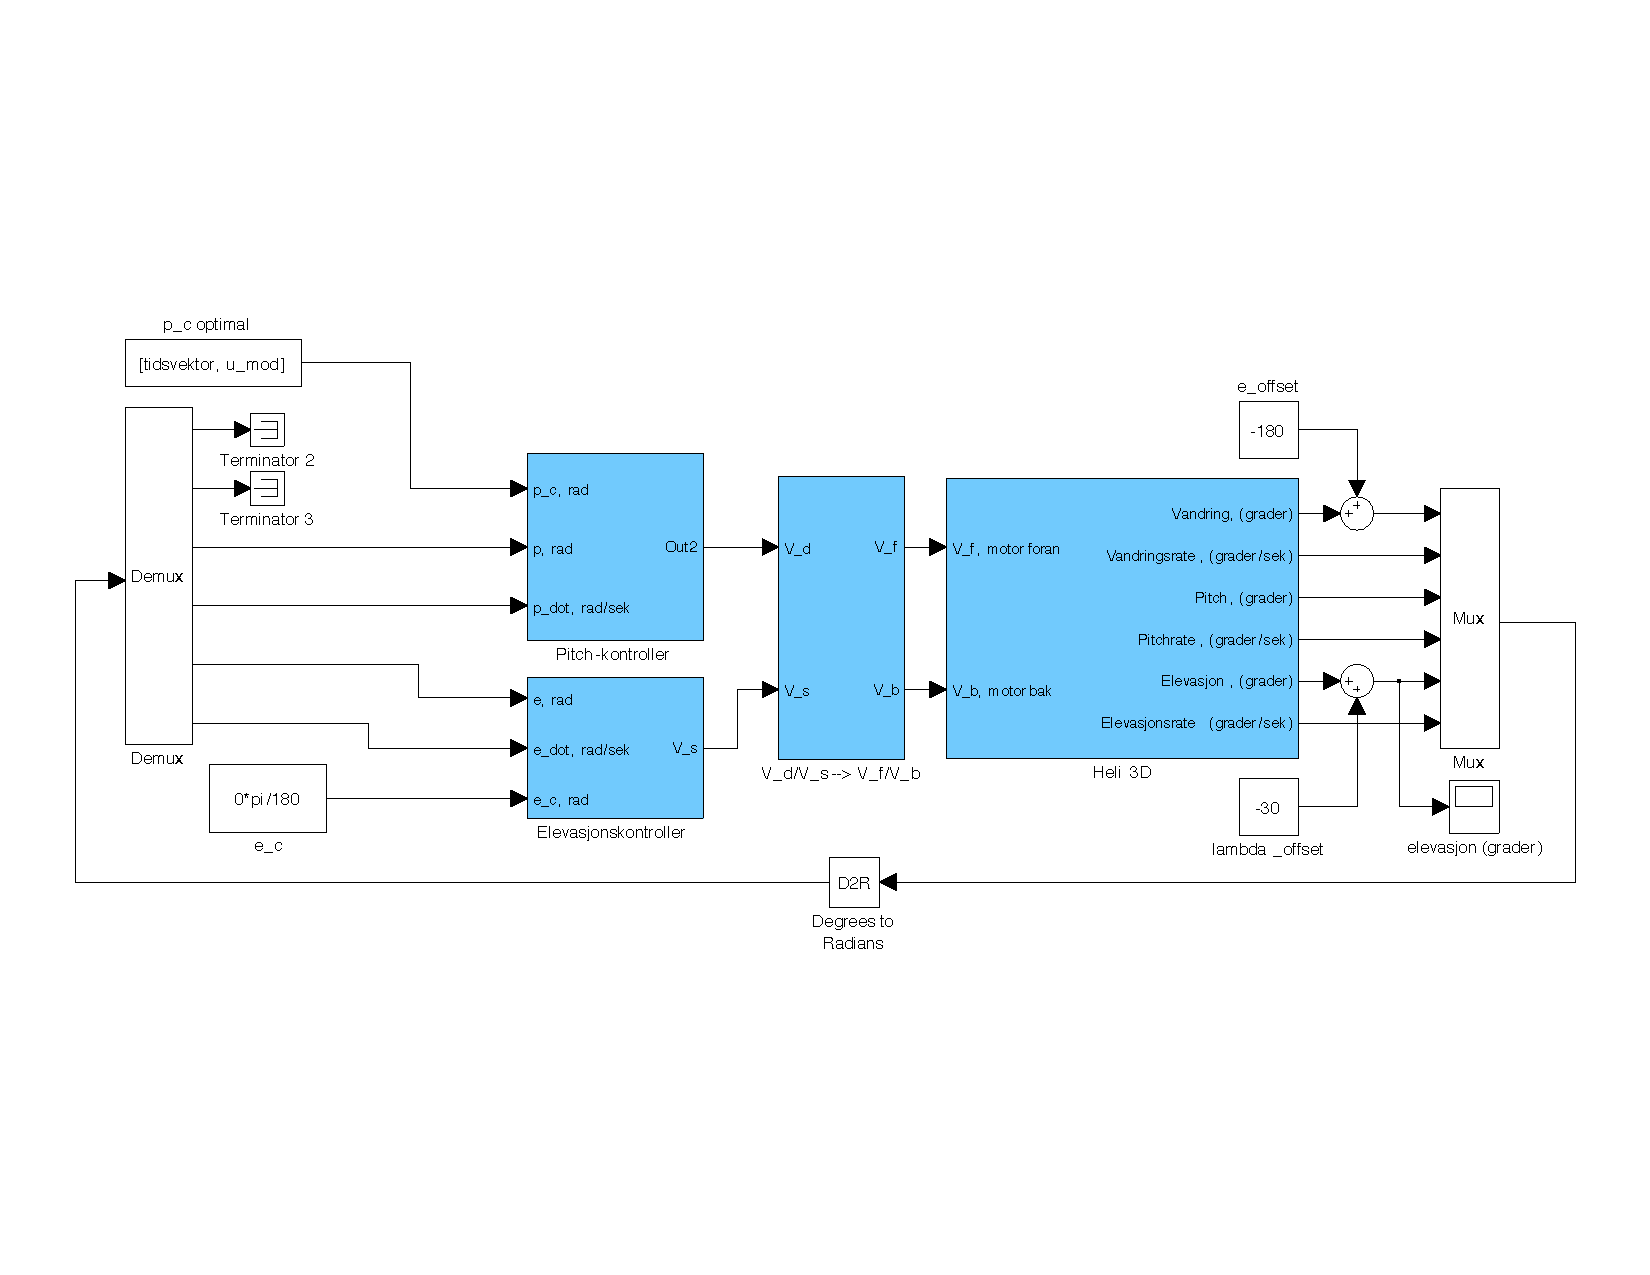
\includegraphics[width = \textwidth]{figures/simulink.pdf}
	\caption{A Simulink diagram.}
\label{fig:simulink}
\end{figure}

\FloatBarrier

\section{Parameters and values}


\begin{table}[tbp]
	\centering
	\caption{Parameters and values.}
	\begin{tabular}{llll}
		\toprule
		Symbol & Parameter & Value & Unit \\
		\midrule
		$l_a$ & Distance from elevation axis to helicopter body & $0.63$  & \meter                      \\
		$l_h$ & Distance from pitch axis to motor               & $0.18$  & \meter                      \\
		$K_f$ & Force constant motor                            & $0.25$  & \newton\per\volt            \\
		$J_e$ & Moment of inertia for elevation                 & $0.83$  & \kilogram\usk\meter\squared \\
		$J_t$ & Moment of inertia for travel                    & $0.83$  & \kilogram\usk\meter\squared \\
		$J_p$ & Moment of inertia for pitch                     & $0.034$ & \kilogram\usk\meter\squared \\
		$m_h$ & Mass of helicopter                              & $1.05$  & \kilogram                   \\
		$m_w$ & Balance weight                                  & $1.87$  & \kilogram                   \\
		$m_g$ & Effective mass of the helicopter                & $0.05$  & \kilogram                   \\
		$K_p$ & Force to lift the helicopter from the ground    & $0.49$  & \newton                     \\
		\bottomrule
	\end{tabular}
\label{tab:parameters}
\end{table}
